\documentclass{standalone}
\usepackage[utf8]{inputenc}
\usepackage{amsmath}
\usepackage{amsfonts}
\usepackage{amssymb}
\usepackage{tikz}
\usetikzlibrary{calc,arrows,positioning,shapes,shapes.gates.logic.US,trees, backgrounds}

\begin{document}


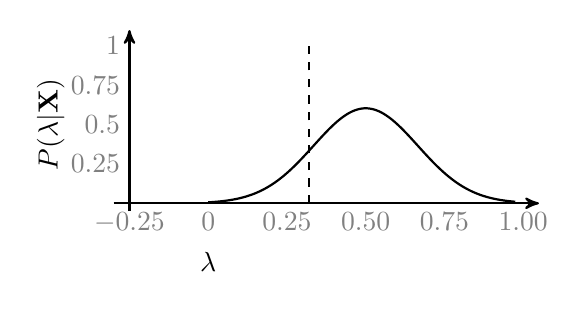
\begin{tikzpicture}[
	scale = 1,
    thick,
        >=stealth',
    dot/.style = {
      draw,
      fill = white,
      circle,
      inner sep = 0pt,
      minimum size = 4pt}
      ]
  % Defining the GRM threshholds curves:  
  \def\gauss{\x, {2/(.5*sqrt(3.5*pi))*exp(-((\x-2)^2)/(3.5*.5^2))}}

  \coordinate (O) at (0,0);

  % X-axis "normal" curve
  \draw[-, domain=0:3.9] plot[samples=1000] (\gauss);
  
  % Draw horizontal grid lines
  \draw[-, very thin,color=gray] (-1,0.5) coordinate[label = {left:$0.25$}] 	-- (-1,0.5) ;
  \draw[-, very thin,color=gray] (-1,1) coordinate[label = {left:$0.5$}] 	-- (-1,1) ;
  \draw[-, very thin,color=gray] (-1,1.5) coordinate[label = {left:$0.75$}] 	-- (-1,1.5) ;
  \draw[-, very thin,color=gray] (-1,2.00)coordinate[label = {left:$1$}]		-- (-1,2) ;
    % Draw Veritcal grid lines
  \draw[-, very thin,color=gray] (-1,0) coordinate[label = {below:$-0.25$}] 	-- (-1,0) ;
  \draw[-, very thin,color=gray] (0,0) coordinate[label = {below:$0$}]	-- (0,0) ;
  \draw[-, very thin,color=gray] (1,0) coordinate[label = {below:$0.25$}]	-- (1,0) ;
  \draw[-, very thin,color=gray] (2,0) coordinate[label = {below:$0.50$}]	-- (2,0) ;
  \draw[-, very thin,color=gray] (3,0) coordinate[label = {below:$0.75$}]	-- (3,0) ;
  \draw[-, very thin,color=gray] (4,0) coordinate[label = {below:$1.00$}]	-- (4,0) ;
  
  \draw[->] (-1.2,0) -- (4.2,0) node(xlab) at (0,-.75) {$\lambda$};
  \draw[->] (-1,-.1) -- (-1,2.2) node[ rotate=90] (ylab) at (-2,1) {$P(\lambda \vert \mathbf{X})$} ;
  
  \draw[-, dashed, color=black] (1.28, 0) to (1.28, 2);
  

\end{tikzpicture}

\end{document}